%%%% Paramétrage du TD %%%%
\def\xxactivite{ \ifprof \normalsize{TD 2 -- Corrigé } \else  \ifcolle Colle \else TD 2\fi \fi} % \normalsize \vspace{-.4cm}
\def\xxauteur{\textsl{Xavier Pessoles}}


\def\xxnumchapitre{Chapitre 1 \vspace{.2cm}}
\def\xxchapitre{\hspace{.12cm} Approche énergétique}

\def\xxcompetences{%
\vspace{-.5cm}
\footnotesize{
\textsl{%
\textbf{Savoirs et compétences :}\\
\vspace{-.2cm}
\begin{itemize}[label=\ding{112},font=\color{ocre}] 
\item Mod2.C18.SF1 : Déterminer l’énergie cinétique d’un solide, ou d’un ensemble de solides, dans son mouvement par rapport à un autre solide.
\item Res1.C1.SF1 : Proposer une démarche permettant la détermination de la loi de mouvement.
%\item Mod1.C5.SF2 : Déterminer la puissance des actions mécaniques extérieures à un solide ou à un ensemble de solides, dans son mouvement rapport à un autre solide.
%\item Mod1.C5.SF3 : Déterminer la puissance des actions mécaniques intérieures à un ensemble de solides.
\end{itemize}}}}


\def\xxtitreexo{Quille pendulaire \ifnormal $\star$ \else \fi \iftdifficile $\star\star\star$ \else \fi }
\def\xxsourceexo{\hspace{.2cm} \footnotesize{Concours Commun Mines Ponts 2014}}

\def\xxfigures{
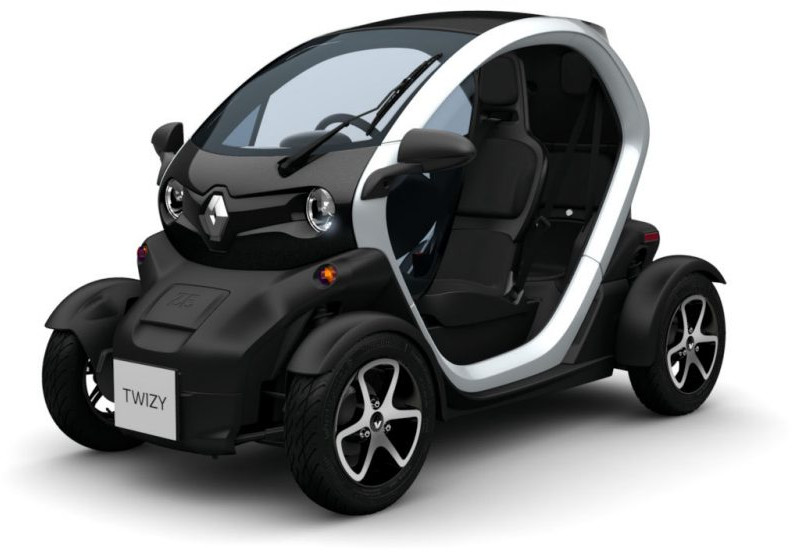
\includegraphics[width=.6\textwidth]{fig_01}
}%figues de la page de garde


\input{\repRel/Style/pagegarde_TD}
\setcounter{numques}{0}

\setlength{\columnseprule}{.1pt}

\pagestyle{fancy}
\thispagestyle{plain}


\vspace{5.2cm}

\def\columnseprulecolor{\color{ocre}}
\setlength{\columnseprule}{0.4pt} 

%%%%%%%%%%%%%%%%%%%%%%%

\setcounter{exo}{0}


\ifprof
%\begin{multicols}{2}
\else
\begin{multicols}{2}
\fi

\section*{Mise en situation}
\ifprof
\else

Les actions de l'air et de l'eau permettent au voilier d'avancer mais provoquent aussi son inclinaison autour de l'axe longitudinal $\vect{z_N}$. C’est le phénomène de gîte. Pour contrebalancer ce mouvement et éviter que le voilier ne se couche sur l’eau, la quille joue le rôle de contrepoids. 


%\begin{center}
%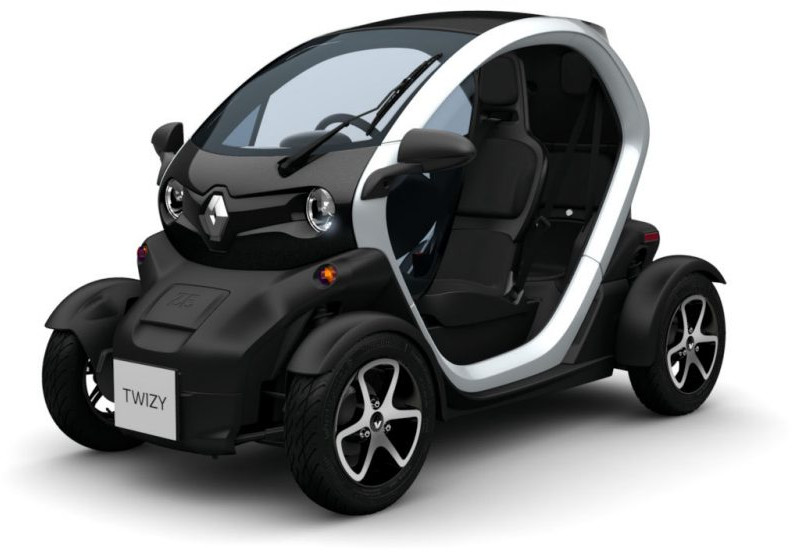
\includegraphics[width=.8\linewidth]{fig_01}
%%\textit{}
%\end{center}

Une évolution récente des voiliers de course océanique a été de les doter d’une quille pendulaire. Cette quille est en liaison pivot d’axe $\left(O,\vect{z}_N \right)$ avec la coque du navire et peut être orientée d’un côté ou de l’autre du navire. Une fois l’orientation désirée obtenue, tout mouvement dans la liaison pivot est supprimé par le blocage en rotation de celle-ci. 

\begin{center}
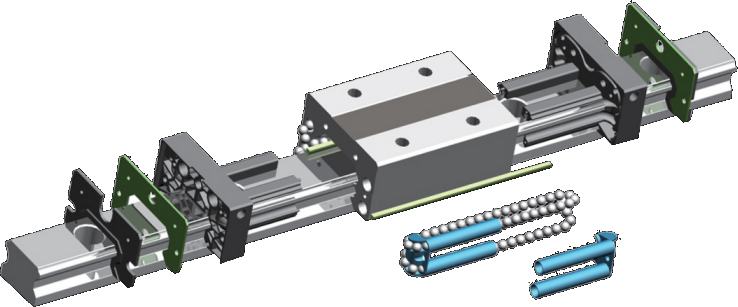
\includegraphics[width=.6\linewidth]{fig_03}

\textit{Modèle volumique 3D}
\end{center}
%Cette quille est généralement constituée d’un voile immergé dans l’eau à l’extrémité duquel se trouve un lest profilé. L’efficacité de la quille dépend de la masse du lest et de la longueur du voile. Ces deux paramètres présentent des limitations : le lest ne peut être trop important sous peine de solliciter dangereusement le voile de quille et la longueur de quille est limitée par le tirant d’eau maximal admissible (il faut permettre l’entrée dans les ports sans toucher le fond !).


%\begin{center}
%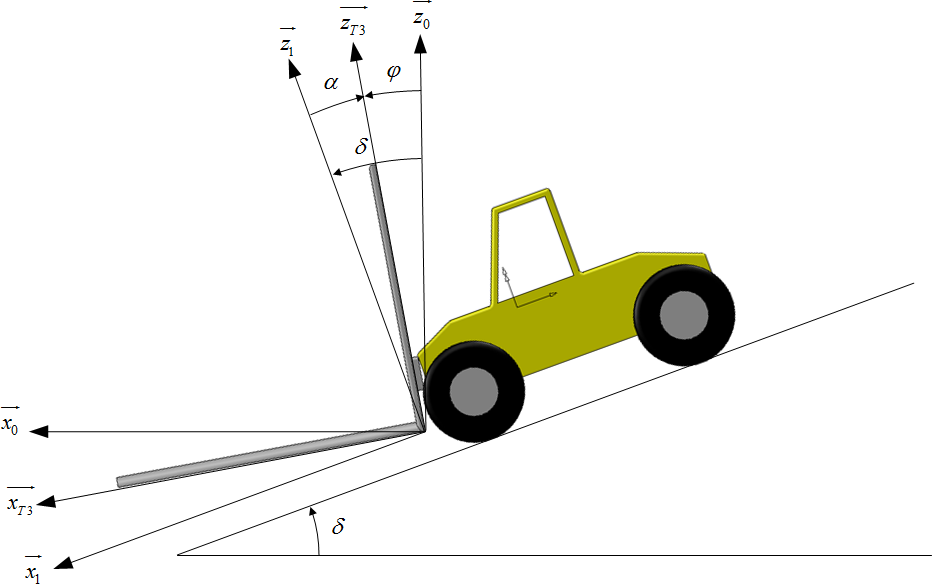
\includegraphics[width=.8\linewidth]{fig_02}
%%\textit{}
%\end{center}


\fi
\begin{obj}
L’objectif est de déterminer la puissance utile au déplacement de la quille et de la comparer à celle installée
par le constructeur.
\end{obj}

\ifprof
\else
%
%\begin{center}
%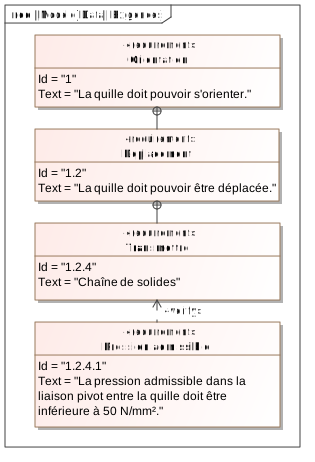
\includegraphics[width=.95\linewidth]{Exigences}
%%\textit{}
%\end{center}

%\subsection*{Travail à réaliser}


\textbf{Hypothèses}

\begin{itemize}
\item Les liaisons sont toutes parfaites.
\item Le bateau est à l’arrêt et son repère $R_N$ est galiléen.
\item Lors de la commande de basculement de la quille, les vérins sont alimentés de telle sorte que : $F_{h2} > 0$ et
$F_{h3} = 0$. Le vérin 2--4 est alors moteur et le vérin 3--5 est libre ($F_{h2}$ désigne l'action hydraulique sur la tige du vérin 2; on a donc $-F_{h2}$ qui agit sur 4).
\item Le mouvement du fluide dans les diverses canalisations s’accompagne d’un phénomène de frottement visqueux défini. L’eau exerce sur le voile de quille une action hydrodynamique.
%\item Seul le vérin 2--4 est moteur ($F_{h3}=0$). Le fluide (pression hydraulique) agit simultanément sur les pièces 2 et 4. L’action du fluide sur 2 est donnée par 
%$\torseurstat{T}{\text{ph}}{2}=\torseurl{F_{h2}\vect{x}_2}{\vect{0}}{C}$.
%\item Les actions mécaniques de frottement visqueux provenant du déplacement du fluide dans les canalisations sont toutes négligées.% ($k=0$).
%\item Les actions hydrodynamiques sur le voile et le lest de quille sont également négligées.
%%\item Les actions hydrodynamiques sur le voile et le lest de quille sont également négligées.
%\item Les poids des éléments constitutifs des deux vérins sont négligés.
%\item La variation de $\theta_2$ pour toute l’amplitude du mouvement de relevage de la quille est faible; $\theta_2$ sera pris égal à 0 : les bases $\mathcal{B}_2$, $\mathcal{B}_4$ et $\mathcal{B}_N$ sont donc confondues. Cependant l’angle $\theta_1$ est différent de zéro.
%\item Les conditions de déplacement rendent négligeables les effets dynamiques. Les théorèmes de la statique seront donc utilisés dans la suite.
\end{itemize}

Le modèle de calcul est donné dans les figures suivantes.

\begin{center}
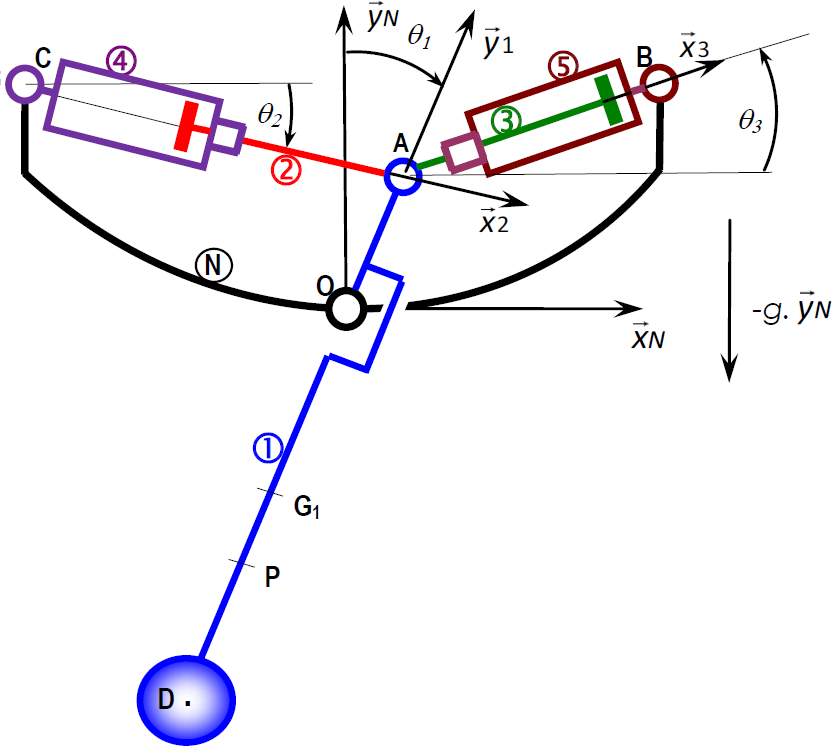
\includegraphics[width=.7\linewidth]{fig_05_a}

\textit{Modèle 2D}
\end{center}

\begin{center}
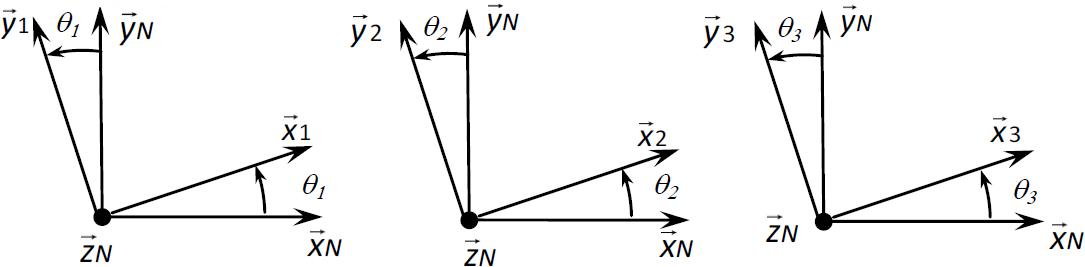
\includegraphics[width=\linewidth]{fig_05_b}

\textit{Paramétrage}
\end{center}

\textbf{Données géométriques, massiques et inertielles}
\begin{multicols}{2}
\footnotesize

$\vect{OA}=R\vect{y_1}$; $\vect{CA}=x_{24}(t)\vect{x_2}$; $\vect{AB}=x_{35}(t)\vect{x_3}$, 
\begin{itemize}
\item Solide 1, masse $M_1$, centre d'inertie $G_1$, $\vect{OG_1}=-L_1\vect{y_1}$, $\inertie{G_1}{1}=\matinertie{A_1}{B_1}{C_1}{-D_1}{0}{0}{\left(\vect{x_1},\vect{y_1},\vect{z_N}, \right)}$.
\item Solide 2, masse $M_2$, centre d'inertie $G_2$, $\vect{AG_2}=-L_2\vect{x_2}$, $\inertie{G_2}{2}=\matinertie{A_2}{B_2}{B_2}{0}{0}{0}{\left(\vect{x_2},\vect{y_2},\vect{z_N}, \right)}$.
\item Solide 3, masse $M_3=M_2$, centre d'inertie $G_3$, $\vect{AG_3}=L_2\vect{x_3}$, $\inertie{G_3}{3}=\matinertie{A_3}{B_3}{B_3}{0}{0}{0}{\left(\vect{x_3},\vect{y_3},\vect{z_N}, \right)}$.
\item Solide 4, masse $M_4$, centre d'inertie $C$, $\inertie{C}{4}=\matinertie{A_4}{B_4}{C_4}{0}{0}{0}{\left(\vect{x_2},\vect{y_2},\vect{z_N}, \right)}$.
\item Solide 5, masse $M_5$, centre d'inertie $B$, $\inertie{B}{5}=\matinertie{A_5}{B_5}{C_5}{0}{0}{0}{\left(\vect{x_3},\vect{y_3},\vect{z_N}, \right)}$.
\end{itemize}
\normalsize

\end{multicols}

\textbf{Actions mécaniques}

\footnotesize
\begin{itemize}
\item Action de pression de l'huile sur 2 : $\torseurstat{T}{\text{ph}}{2}=\torseurl{F_{h2}\vect{x_2}}{\vect{0}}{C}$.
\item Action de pression de l'huile sur 3 : $\torseurstat{T}{\text{ph}}{3}=\torseurl{-F_{h3}\vect{x_3}}{\vect{0}}{B}$.
\item Action de frottement visqueux de l'huile sur 2 : $\torseurstat{T}{\text{phf}}{2}=\torseurl{-k\dfrac{\dd x_{24}(t)}{\dd t}\vect{x_2}}{\vect{0}}{A}$ avec $k>0$.
\item Action de frottement visqueux de l'huile sur 3 : $\torseurstat{T}{\text{phf}}{3}=\torseurl{-k\dfrac{\dd x_{35}(t)}{\dd t}\vect{x_3}}{\vect{0}}{A}$ avec $k>0$.
\item Action hydraudynamique de l'eau sur 1 : $\torseurstat{T}{\text{eau}}{1}=\torseurl{F_p\vect{z_1}+F_t\vect{x_1}}{\vect{0}}{P}$ avec $\vect{OP}=-h\vect{y_1}$.
\end{itemize}

\normalsize
%
%\begin{center}
%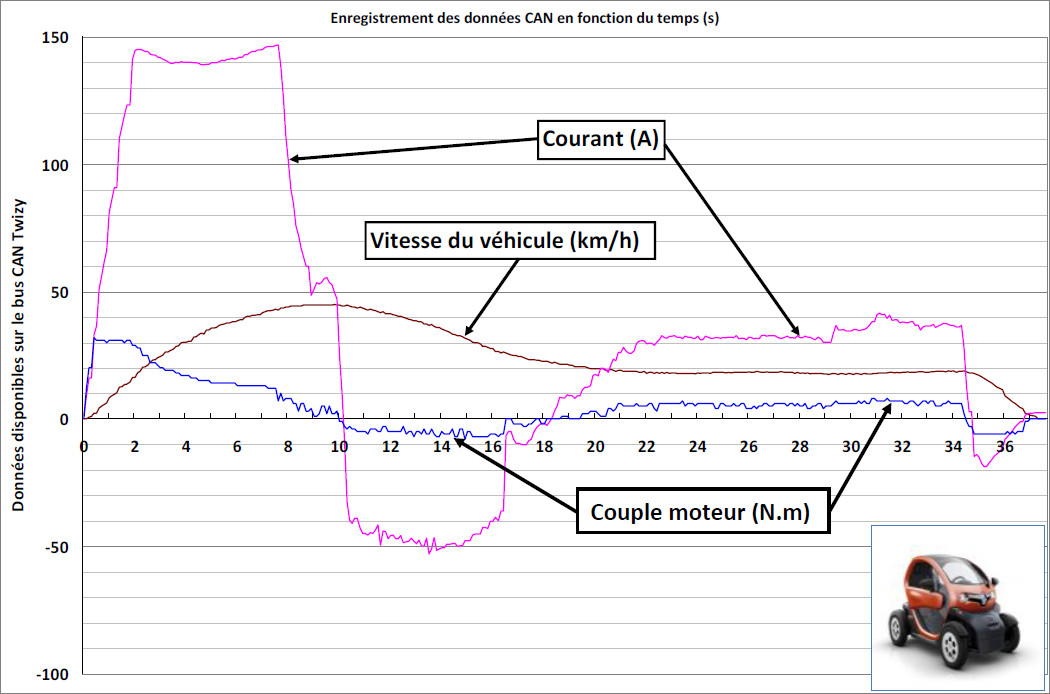
\includegraphics[width=\linewidth]{fig_04}
%
%%\vspace{-.2cm}
%
%$\vect{OA}=R\vect{y_1}$, 
%$\theta_1 =\angl{x_N}{x_1}$,
%$\vect{OG_1}=-L_1\vect{y_1}$,
%$\vect{AA_2}=-d\vect{z_N}$
%$\vect{AA_3}=d\vect{z_N} $.
%
%%\vspace{-.8cm}
%
%\textit{Schéma cinématique 3D}
%\end{center}




\fi



\ifnormal

\subsection*{Vecteurs vitesse}

\question{Tracer le graphe de liaisons.}
\ifprof
\begin{corrige} ~\\

\begin{center}
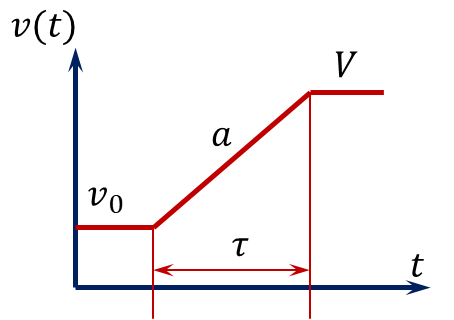
\includegraphics[width=.45\linewidth]{cor_01}
\end{center}
\end{corrige}
\else
\fi



\question{
Exprimer les vitesses suivantes :
\begin{enumerate}
\item $\vectv{G_1}{1}{N}$ en fonction de $\dfrac{\dd \theta_1(t)}{\dd t}$ et des paramètres géométriques utiles;
\item $\vectv{G_2}{2}{N}$ en fonction de $\dfrac{\dd \theta_2(t)}{\dd t}$, $\dfrac{\dd x_{24}(t)}{\dd t}$, $x_{24}$ et des paramètres géométriques utiles;
\item $\vectv{G_3}{3}{N}$ en fonction de $\dfrac{\dd \theta_3(t)}{\dd t}$, $\dfrac{\dd x_{35}(t)}{\dd t}$, $x_{35}$ et des paramètres géométriques utiles;
\item $\vectv{A}{2}{4}$ en fonction de  $\dfrac{\dd x_{24}(t)}{\dd t}$.
\end{enumerate}}
\ifprof
\begin{corrige}~\\
\begin{enumerate}
\item $\vectv{G_1}{1}{N}=\vectv{O}{1}{N}+\vect{G_1 O}\wedge \vecto{1}{N}=$ $L_1\vect{y_1}\wedge \dot{\theta}_1\vect{z_N}$ $=L_1 \dot{\theta}_1\vect{x_1}$.
\item $\vectv{G_2}{2}{N}=$ $\left[  \dfrac{\dd \left( \vect{OA} + \vect{AG_2}\right)}{\dd t}\right]_{R_N}$ 
$=\left[ \dfrac{\dd \left( R\vect{y_1}  -L_2 \vect{x_2}\right)}{\dd t}\right]_{R_N}$ $= -R\dot{\theta}_1\vect{x_1}  -L_2 \dot{\theta}_2\vect{y_2}$. 

On a aussi $\vectv{G_2}{2}{N}=$ $\left[  \dfrac{\dd \left( \vect{CA} + \vect{AG_2}\right)}{\dd t}\right]_{R_N}$ 
$=\left[ \dfrac{\dd \left(  x_{24}(t)\vect{x_2}  -L_2 \vect{x_2}\right)}{\dd t}\right]_{R_N}$ $=  \dot{x}_{24}(t)  \vect{x_2}+\dot{\theta}_2\left(  x_{24}(t)  -L_2 \right)\vect{y_2}$.

\item $\vectv{G_3}{3}{N}$  $=\left[  \dfrac{\dd \left( \vect{OA} + \vect{AG_3}\right)}{\dd t}\right]_{R_N}$ 
$=\left[ \dfrac{\dd \left( R\vect{y_1} + L_2 \vect{x_3}\right)}{\dd t}\right]_{R_N}$ $= -R\dot{\theta}_1\vect{x_1}  +L_2 \dot{\theta}_3\vect{y_3}$. 


On a aussi $\vectv{G_3}{3}{N}=$ $\left[  \dfrac{\dd \left( \vect{BA} + \vect{AG_3}\right)}{\dd t}\right]_{R_N}$ 
$=\left[ \dfrac{\dd \left(  -x_{35}(t)\vect{x_3}  +L_2 \vect{x_3}\right)}{\dd t}\right]_{R_N}$ $= - \dot{x}_{35}(t)  \vect{x_3}+\dot{\theta}_3\left(  -x_{35}(t)  +L_2 \right)\vect{y_3}$.


\item $\vectv{A}{2}{4}$ $=\left[  \dfrac{\dd  \vect{CA} }{\dd t}\right]_{R_4}$  $=\left[  \dfrac{\dd \left( x_{24}(t)\vect{x_2} \right)}{\dd t}\right]_{R_4}$ $= \dot{x}_{24}(t)\vect{x_2}$.
\end{enumerate}
\end{corrige}
\else
\fi

\subsection*{Energie cinétique}
Soit $E$ l’ensemble constitué des solides 1, 2, 3, 4 et 5.

On note $\ec{i}{N}$ l'énergie cinétique de $i$ dans son mouvement par rapport au référentiel galiléen $R_N$.

\question{
Exprimer les énergies cinétiques suivantes : 
\begin{enumerate}
\item $\ec{1}{N}$, en fonction de
$\dfrac{\dd \theta_1(t)}{\dd t}$  et des paramètres inertiels et géométriques utiles;
\item $\ec{2}{N}$, en fonction de
$\dfrac{\dd \theta_2(t)}{\dd t}$ , $\dfrac{\dd x_{24}(t)}{\dd t}$ , $x_{24}(t)$ et des paramètres inertiels et géométriques utiles.
\item $\ec{4}{N}$, en fonction de $\dfrac{\dd \theta_2(t)}{\dd t}$ et des paramètres inertiels et géométriques utiles.
\end{enumerate}}
\ifprof
\begin{corrige}~\\
\begin{enumerate}
\item $\ec{1}{N}=\dfrac{1}{2}\torseurcin{V}{1}{N}\otimes \torseurci{1}{N}$ 
$=\dfrac{1}{2}\torseurl{\vecto{1}{N}}{\vectv{G_1}{1}{N}}{G_1}\otimes \torseurl{M_1\vectv{G_1}{1}{N}}{\vectmc{G_1}{1}{N}}{G_1}$
$=\dfrac{1}{2}\torseurl{\dot{\theta}_1\vect{z_N}}{L_1 \dot{\theta}_1\vect{x_1}}{G_1}\otimes \torseurl{M_1L_1 \dot{\theta}_1\vect{x_1}}{\dot{\theta}_1\left(-D_1\vect{y_N}+C_1\vect{z_N}\right) }{G_1}$ $=\dfrac{1}{2}\left(\dot{\theta}_1^2\left(-D_1\vect{y_N}+C_1\vect{z_N}\right)\vect{z_N} + M_1L_1^2 \dot{\theta}_1^2 \right)$
$=\dfrac{1}{2}\left(\dot{\theta}_1^2C_1 + M_1L_1^2 \dot{\theta}_1^2 \right)$
$=\dfrac{1}{2}\dot{\theta}_1^2\left(C_1 + M_1L_1^2  \right)$.

\item $\ec{2}{N}=\dfrac{1}{2}\torseurcin{V}{2}{N}\otimes \torseurci{2}{N}$ 
$=\dfrac{1}{2}\torseurl{\vecto{2}{N}}{\vectv{G_2}{2}{N}}{G_2}\otimes \torseurl{M_2\vectv{G_2}{2}{N}}{\vectmc{G_2}{2}{N}}{G_2}$

$=\dfrac{1}{2}
\torseurl{\dot{\theta}_2\vect{z_N}}{\dot{x}_{24}(t)  \vect{x_2}+\dot{\theta}_2\left(  x_{24}(t)  -L_2 \right)\vect{y_2}}{G_2}
\otimes 
\torseurl{M_2\left(\dot{x}_{24}(t)  \vect{x_2}+\dot{\theta}_2\left(  x_{24}(t)  -L_2 \right)\vect{y_2}\right)}{\dot{\theta}_2 B_2 \vect{z_N} }{G_1}
$ 

$=\dfrac{1}{2}\left( B_2 \dot{\theta}_2^2 +M_2\left(\dot{x}_{24}(t)  \vect{x_2}+\dot{\theta}_2\left(  x_{24}(t)  -L_2 \right)\vect{y_2}\right)^2  \right)
$ 
$=\dfrac{1}{2}\left( B_2 \dot{\theta}_2^2 +M_2\left(\dot{x}_{24}(t)^2+\dot{\theta}_2^2\left(  x_{24}(t)  -L_2 \right)^2\right)  \right)
$ 
.
\item $\ec{4}{N}=\dfrac{1}{2}C_4\dot{\theta}_2^2$ . 
\end{enumerate}
\end{corrige}
\else
\fi


\subsection*{Evaluation des puissances développées par les actions mécaniques intérieures à E}
\question{Recenser, puis exprimer les puissances non nulles (notées $\pint{i}{j}{}$) développées par les actions mécaniques intérieures à $E$ en fonction du (ou des) paramètre(s) propre(s) à la liaison ou au mouvement concerné.}
\ifprof
\begin{corrige} ~\\

Bilan des puissances intérieures à l'ensemble 1, 2, 3, 4, 5 :
\begin{itemize}
\item la puissance dissipée dans les liaisons est nulle car il n'y a pas de frottements;
\item  $\pint{4}{2}{Ph} = \torseurstat{T}{4}{2}\otimes \torseurcin{V}{2}{4}$ 
$=\torseurl{\vectf{4}{2}}{\vectm{A}{4}{2}}{A}\otimes \torseurl{\vecto{2}{4}}{\vectv{A}{2}{4}}{A}$ 

 $=\torseurl{\vectf{4}{2}}{-}{A}\otimes \torseurl{\vect{0}}{\vectv{A}{2}{4}}{A}$
  $=\torseurl{F_{h2}\vect{x_2}}{-}{A}\otimes \torseurl{\vect{0}}{ \dot{x}_{24}(t)  \vect{x_2}}{A}$
  $=F_{h2}\dot{x}_{24}$;

  \item  $\pint{4}{2}{Phf}  $
 $=\torseurl{\vectf{4}{2}}{-}{A}\otimes \torseurl{\vect{0}}{\vectv{A}{2}{4}}{A}$
  $=\torseurl{-k\dot{x}_{24}(t)  \vect{x_2}}{-}{A}\otimes \torseurl{\vect{0}}{ \dot{x}_{24}(t)  \vect{x_2}}{A}$  $=-k\dot{x}_{24}^2(t)$;
\item  $\pint{3}{5}{Ph}  $
$=\torseurl{\vectf{5}{3}}{-}{A}\otimes \torseurl{\vect{0}}{\vectv{A}{3}{5}}{A}$
$=\torseurl{F_h  \vect{x_3}}{-}{A}\otimes \torseurl{\vect{0}}{ \dot{x}_{35}(t)  \vect{x_3}}{A}$ $=F_h\dot{x}_{35}(t)$;
\item  $\pint{3}{5}{Phf}  $
$=\torseurl{\vectf{5}{3}}{-}{A}\otimes \torseurl{\vect{0}}{\vectv{A}{3}{5}}{A}$
$=\torseurl{-k\dot{x}_{35}(t)  \vect{x_3}}{-}{A}\otimes \torseurl{\vect{0}}{ \dot{x}_{35}(t)  \vect{x_3}}{A}$ $=-k\dot{x}_{35}^2(t)$.
\end{itemize}

\end{corrige}
\else
\fi


\subsection*{Evaluation des puissances développées par les actions mécaniques extérieures à E}
\question{Recenser, puis exprimer les puissances galiliéennes non nulles (notées $\pext{i}{j}{k}$) développées par les actions mécaniques extérieures à $E$. Chaque puissance sera exprimée à l’aide du (ou des)
paramètre(s) propre(s) à la liaison ou au mouvement concerné.}
\ifprof
\begin{corrige}
Bilan des puissances intérieures à l'ensemble 1, 2, 3, 4, 5 :
\begin{itemize}
\item la puissance dissipée dans les liaisons est nulle car il n'y a pas de frottements;
\item  $\pext{\text{pes}}{1}{R_N} = \torseurstat{T}{\text{pes}}{1}\otimes \torseurcin{V}{1}{R_N}$ 
$=\torseurl{-M_1g\vect{y_N}}{0}{G_1}\otimes \torseurl{\dot{\theta}_1\vect{z_N}}{\vectv{G_1}{1}{R_N}=L_1 \dot{\theta}_1\vect{x_1}}{G_1}$ 

 $=-M_1gL_1 \dot{\theta}_1\vect{x_1}\vect{y_N}$ $=-M_1gL_1 \dot{\theta}_1\sin \theta_1$;

\item  $\pext{\text{pes}}{2}{R_N} = \torseurstat{T}{\text{pes}}{2}\otimes \torseurcin{V}{2}{R_N}$ 
$=\torseurl{-M_2g\vect{y_N}}{0}{G_2}\otimes \torseurl{\dot{\theta}_1\vect{z_N}}{ \dot{x}_{24}(t)  \vect{x_2}+\dot{\theta}_2\left(  x_{24}(t)  -L_2 \right)\vect{y_2}}{G_1}$ 

 $= -M_2g\vect{y_N}\left(\dot{x}_{24}(t)  \vect{x_2}+\dot{\theta}_2\left(  x_{24}(t)  -L_2 \right)\vect{y_2}\right)$ $= -M_2g\dot{x}_{24}(t) \sin \theta_2-M_2g\dot{\theta}_2\left(  x_{24}(t)  -L_2 \right)\cos \theta_2$;

\item  $\pext{\text{pes}}{3}{R_N} $
 $= -M_3g\vect{y_N}\left(-\dot{x}_{35}(t)  \vect{x_3}+\dot{\theta}_3\left( - x_{35}(t)  +L_2 \right)\vect{y_3}\right)$
 
  $= -M_3g\left(-\dot{x}_{35}(t)  \sin\theta_3+\dot{\theta}_3\left( - x_{35}(t)  +L_2 \right)\cos\theta_3\right)$ ;
 
  
\item  $\pext{\text{eau}}{1}{R_N} = \torseurstat{T}{\text{eau}}{1}\otimes \torseurcin{V}{1}{R_N}$ 
$=\torseurl{F_p \vect{z_1}+F_t \vect{x_1}}{0}{P}\otimes \torseurl{\dot{\theta}_1\vect{z_N}}{h \dot{\theta}_1\vect{x_1}}{P}$ 

$=F_t h \dot{\theta}_1$;
% $=-MgL_1 \dot{\theta}_1\vect{x_1}\vect{y_N}$ $=-MgL_1 \dot{\theta}_1\sin \theta_1$;

\end{itemize}
\end{corrige}
\else
\fi

\question{Appliquer le théorème de l’énergie-puissance à $E$ dans son mouvement par rapport à $N$. Écrire ce
théorème de façon globale en utilisant uniquement les notations précédentes, sans leur
développement. Exprimer dans ces conditions la puissance motrice que fournit le vérin moteur en
fonction du reste : équation (1).}
\ifprof
\begin{corrige}
On a :
$\pext{\bar{E}}{E}{R_N} + \sum \pint{i}{j}{}=\dfrac{\dd \ec{E}{R_N}}{\dd t}$
\end{corrige}
\else
\fi

\else
\fi


\iftdifficile

\question{ Exprimer la puissance motrice que fournit le vérin moteur en
fonction des données du problème. La méthode sera précisément décrite. Chacun des termes seront calculés. Il n'est pas demandé d'écrire la relation finale.}
\else
\fi

\ifprof
\else


On se place dans le cas où une commande en vitesse est générée à destination du vérin [2, 4]. Le vérin [3, 5]
est libre. Cette commande <<~en trapèze de vitesse~>>  provoque le déplacement de la quille de la position $\theta_1=0$
 à la position $\theta_1 = 45\degres$ en 4 secondes, le maintien de la quille dans cette position pendant 1 seconde puis le
 retour à la position $\theta_1=0$ en 4 secondes. Les phases d’accélération et de décélération (rampes) durent 1 seconde.


\begin{center}
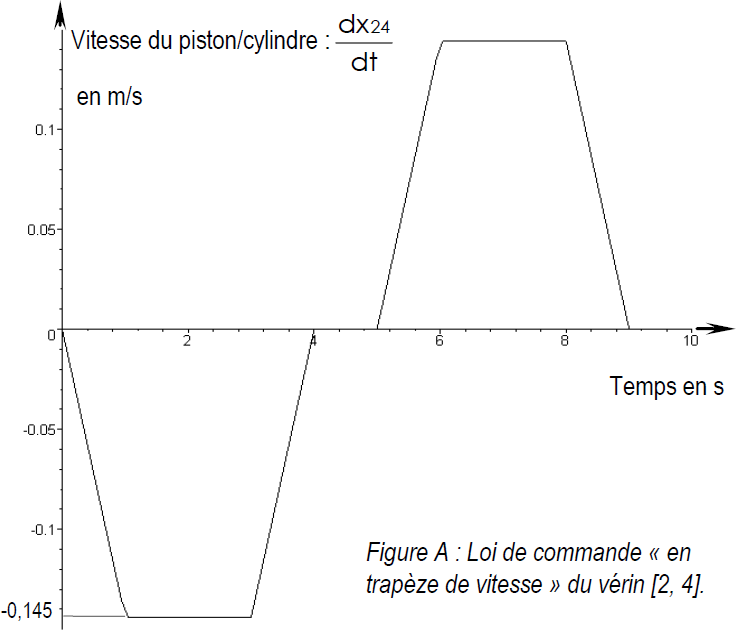
\includegraphics[width=.6\linewidth]{fig_06}
%\textit{Paramétrage}
\end{center}

Un logiciel de calcul permet de tracer l’évolution temporelle des puissances mises en jeu. Ces puissances sont
représentées sur la figure suivante. 

\begin{center}
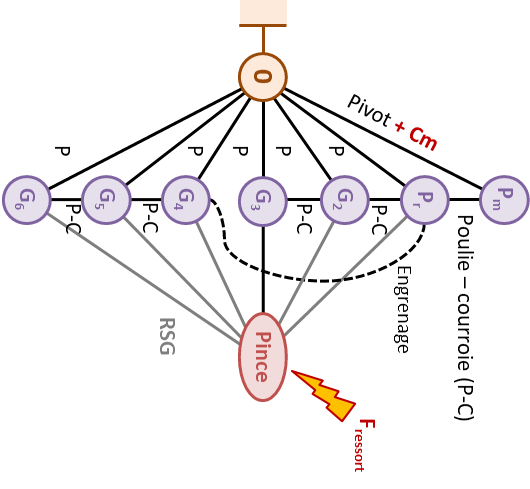
\includegraphics[width=.8\linewidth]{fig_07}
%\textit{Paramétrage}
\end{center}

\fi

\question{Dans le but de chiffrer la valeur maximale de la puissance que doit fournir l’actionneur pour réaliser
le mouvement prévu, tracer, à l’aide de la figure précédente, l’allure de
l’évolution temporelle de cette puissance. Pour cela, évaluer les valeurs aux instants $t=\SI{0}{s}$, $t=\SI{1}{s}$,
$t=\SI{3}{s}$ et $t=\SI{4}{s}$.
Sur cet intervalle $[0,\SI{4}{s}]$, évaluer, en kW, la valeur maximale de la puissance que doit fournir
l’actionneur. Expliquer pourquoi le maximum de puissance est situé sur cet intervalle.}
\ifprof
\begin{corrige}
D'après UPSTI. À \SI{1}{s}, $2200+5800+2500+4000=\SI{14500}{W}$ à \SI{3}{s}
$0+4000+2500+16000=\SI{22500}{W}$
Maximum à environ \SI{22,5}{kW}.
Le maximum est bien sur cet intervalle car le poids y est résistant (le poids est moteur sur
[\SI{5}{s} ; \SI{8}{s}]).

\end{corrige}
\else
\fi
\question{
Le constructeur indique une puissance motrice installée sur son bateau de \SI{30}{kW}.
Dans les hypothèses utilisées pour constituer le modèle de calcul, indiquer ce qui peut expliquer la
différence entre la valeur calculée et la valeur installée.}
\ifprof
\begin{corrige}
D'après UPSTI. La différence est de \SI{7,5}{kW}.
Elle ne peut pas provenir des hypothèses faites (liaisons parfaites et RN galiléen).
Elle provient certainement du fait que le système est surdimensionné
pour pallier les erreurs de modélisation des actions de l'eau, le vieillissement de la quille avec
les algues collées qui rajoutent du poids...
\end{corrige}
\else
\fi


\ifprof
%\end{multicols}
\else
\end{multicols}
\fi


